\documentclass{standalone}
\RequirePackage{tikz}
\RequirePackage{ifthen}
\usetikzlibrary{arrows,shapes}
\tikzstyle{btreeptr} = [draw, ultra thin, fill=blue!50, minimum height=1cm, inner sep=0cm, minimum width=0cm]
\tikzstyle{btreeval} = [draw, semithick, fill=yellow!30, minimum size=1cm]
\tikzstyle{btlink} = [draw, thick, ->, >=triangle 45]
\newcommand{\xyshift}[3]{
  \begin{scope}[xshift=#1, yshift=#2]
    #3
  \end{scope}
}
\newcommand{\btreelink}[2]{
\draw[btlink] (#1.south) -- ([yshift=-0.1cm] #2.north); \&
\fill (#1.south) circle[radius=0.15cm]; \\
}
\newcommand{\btreenodea}[2]{
\matrix [ampersand replacement=\&] (#1)
{
 \node[btreeptr] (#1-a) {\vphantom{1}}; \& \node[btreeval] {#2}; \&
 \node[btreeptr] (#1-b) {\vphantom{1}}; \\
};
}
\newcommand{\btreenodeb}[3]{
\matrix [ampersand replacement=\&] (#1)
{
 \node[btreeptr] (#1-a) {\vphantom{1}}; \& \node[btreeval] {#2}; \&
 \node[btreeptr] (#1-b) {\vphantom{1}}; \& \node[btreeval] {#3}; \&
 \node[btreeptr] (#1-c) {\vphantom{1}}; \\
};
}

\begin{document}
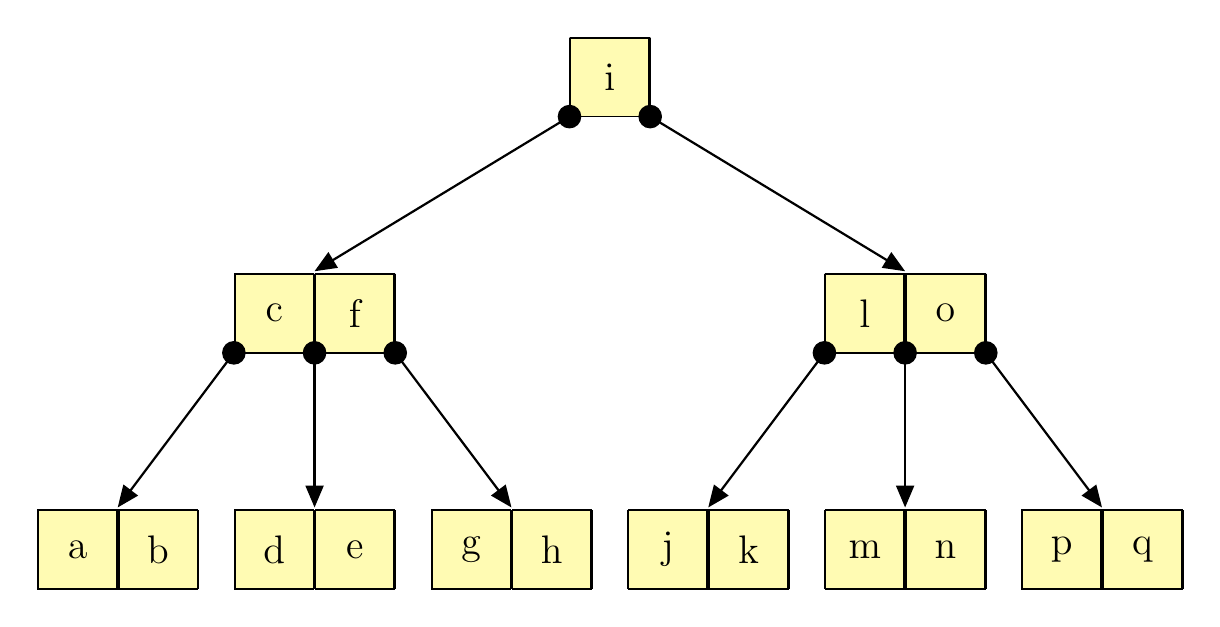
\begin{tikzpicture}
\tikzstyle{every node}=[font=\fontsize{15}{0}\selectfont]
\xyshift{12.5mm}{-60mm}{\btreenodeb{c}{a}{b}}
\xyshift{37.5mm}{-60mm}{\btreenodeb{e}{d}{e}}
\xyshift{62.5mm}{-60mm}{\btreenodeb{g}{g}{h}}
\xyshift{87.5mm}{-60mm}{\btreenodeb{i}{j}{k}}
\xyshift{112.5mm}{-60mm}{\btreenodeb{ba}{m}{n}}
\xyshift{137.5mm}{-60mm}{\btreenodeb{bc}{p}{q}}
\xyshift{37.5mm}{-30mm}{\btreenodeb{b}{c}{f}}
\xyshift{112.5mm}{-30mm}{\btreenodeb{h}{l}{o}}
\xyshift{75mm}{0mm}{\btreenodea{a}{i}}


\btreelink{b-a}{c}
\btreelink{b-b}{e}
\btreelink{b-c}{g}
\btreelink{h-a}{i}
\btreelink{h-b}{ba}
\btreelink{h-c}{bc}
\btreelink{a-a}{b}
\btreelink{a-b}{h}
\end{tikzpicture}
\end{document}
